\documentclass{article}

\usepackage{graphicx}
\usepackage{epsfig}
\usepackage{float}
\usepackage{booktabs}
\usepackage{hyperref}

\title{Olorin}
\author{James Morris (\texttt{jm20@sanger.ac.uk})\\
Jeffrey Barrett (\texttt{barrett@sanger.ac.uk})}
\date{\today}

\begin{document}

\maketitle

\section{Introduction}

Olorin is a tool which integrates gene flow output from Merlin and next generation sequencing data. Users can interactively filter and prioritize variants based on haplotype sharing across different sets of selected individuals and allele frequency in reference datasets.

\section{Getting started with Olorin}
	\subsection{Installing and launching}
		To start you will need Java 6.0 (also known as version 1.6) or newer on your computer. Click \href{http://www.java.com/getjava/}{here} to get the latest version of Java.\\
		
		\noindent First unzip the \texttt{Olorin.zip} file, this directory should contain the following files and directories:
		\begin{itemize}
			\item{\texttt{Olorin.jar} - The application}
			\item{\texttt{lib/} - Required software libraries}
			%\item{\texttt{example/} - Example input data}
			%\item{\texttt{Olorin-help.pdf} - Software manual}
		\end{itemize}
		Once decompressed you can move the \texttt{Olorin.jar} to any desired location, however you also need to ensure that you move the \texttt{lib/} directory as well.\\

		\noindent You can launch Olorin by simply double clicking the \texttt{Olorin.jar} file, this will start the program with the system default amount of memory which may be insufficient for larger data sets. To launch Olorin with more memory use the command line and the following command:
\begin{verbatim}
java -jar Olorin.jar -Xmx 1024m 
\end{verbatim}
This will launch Olorin with up to 1Gb of memory available, to increase this amount further simply change the value passed to the \texttt{-Xmx} argument.

\section{Loading data}
\subsection{Input file formats}
Olorin requires 4 input file types:
\begin{itemize}
	\item{.flow}\\
	Estimated haplotypes should be input as \texttt{.flow} files, generated using \href{http://www.sph.umich.edu/csg/abecasis/Merlin/}{MERLIN}. The \texttt{.flow} file format is described \href{http://www.sph.umich.edu/csg/abecasis/Merlin/tour/haplotyping.html}{here}. Olorin requires the \texttt{.flow} files to be in the horizontal format for outputting haplotypes, this is achieved simply by passing \href{http://www.sph.umich.edu/csg/abecasis/Merlin/reference.html}{MERLIN} the \texttt{--horizontal} flag along with your command. The \texttt{.flow} files should be split by chromosome with the files named using the following format: fam.22.flow (for chromosome 22).
	\item{.map}\\
	The genomic position of each marker used to generate the estimated haplotypes is loaded into Olorin using \texttt{.map} files. The \texttt{.map} file format is described \href{http://pngu.mgh.harvard.edu/~purcell/plink/data.shtml#map}{here}. The \texttt{.map} files should also be split by chromosome with the files named using the following format: fam.22.map (for chromosome 22).
	\item{.ped}\\
	Pedigree information should be described in a single \texttt{.ped} file. The \texttt{.ped} file format is described \href{http://pngu.mgh.harvard.edu/~purcell/plink/data.shtml#ped}{here}.
	\item{.vcf}\\
	The variants from all the sequenced individuals in the pedigree should be contained in a single Varaint Call Format (VCF) file (version 4.0 or greater) which has been compressed using bgzip and indexed using \href{http://samtools.sourceforge.net/tabix.shtml}{tabix}. In cases where you have more than one VCF file, a single VCF can be created using the \texttt{vcf-merge} function of \href{http://vcftools.sourceforge.net/}{VCFtools}. The \texttt{.vcf} file format is described in more detail \href{http://www.1000genomes.org/node/101}{here}.
\end{itemize}

All the previously described file types should be contained in one directory for each pedigree. If, for instance, you had data from a pedigree named \texttt{fam} from chromosomes 20-22, your directory would have files as follows:

\begin{verbatim}
fam.ped
fam.vcf.gz
fam.vcf.gz.tbi
fam.20.flow fam.20.map
fam.21.flow fam.21.map
fam.22.flow fam.22.map
\end{verbatim}

\subsection{Opening a data directory}
To open a data directory select \texttt{Open directory} from the \texttt{File} menu and select its location on the file system.

\section{The user interface}
\begin{figure}[H]
	\centering
		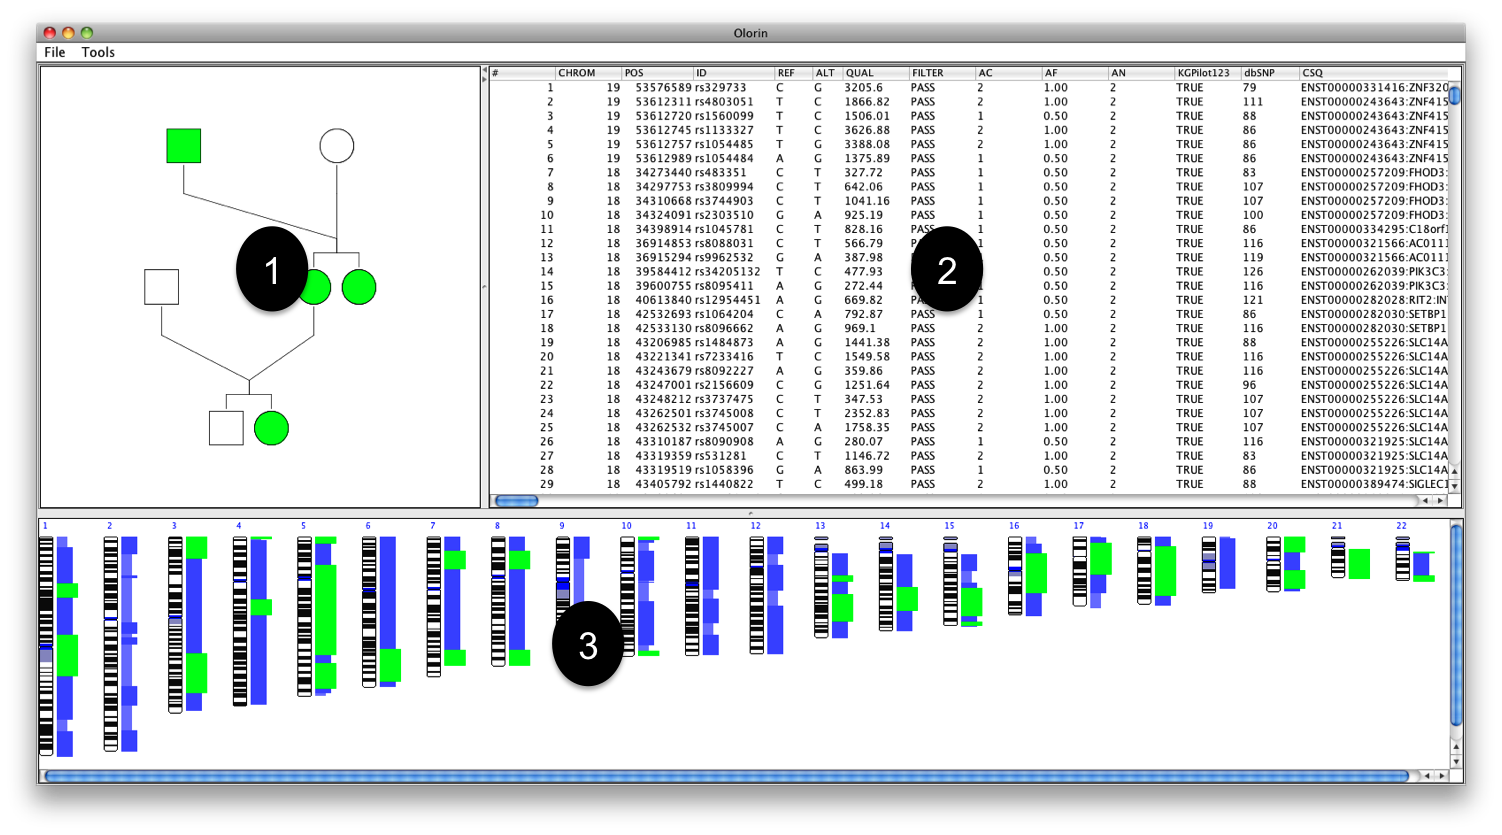
\includegraphics[scale=0.5]{olorin_main}
	\caption{The Olorin user interface.}
	\label{main}
\end{figure}
\begin{enumerate}
	\item{The pedigree panel}
		\begin{itemize}
			\item{The pedigree panel automatically draws an interactive pedigree from the information contained in the \texttt{.ped} file.}
			\item{More information about each individuals in the pedigree can be obtained by hovering a mouse over any node to display the individual, maternal and paternal IDs of the node.}
			\item{Individuals in the pedigree which are male are drawn as squares and females as circles.}
			\item{Affected individuals in the pedigree are shown using filled symbols and unaffected individuals are unfilled.}
			\item{To select or unselect any individual in the pedigree simply click on the node in the pedigree, selected individuals are shown highlighted in green.}
		\end{itemize}
	\item{The variants panel}
		\begin{itemize}
			\item{The variants panel displays all the variants from the \texttt{VCF} which pass the filtering criteria that has been set.}
			\item{The table of variants can be sorted on any of the columns by simply clicking on the column heading.}
		\end{itemize}
	\item{The genome wide sharing panel}
		\begin{itemize}
			\item{The genome wide sharing plots show all the regions shared by the currently selected individuals across the genome.}
			\item{The shade and height of each region reflects the number of chromosomes shared at that position across in genome.}
			\item{Regions which are greater than or equal to the minimum matching chromosomes threshold set by the user are coloured in green.}
		\end{itemize}	
\end{enumerate}

\section{Filtering variants}
\begin{itemize}
	\item{To filter variants first select the individuals in the pedigree you wish to filter on by clicking on them so they become highlighted.}
	\item{Once all the desired individuals have been highlighted, select \texttt{Find Segments} from the \texttt{Tools} menu, a filtering window will then be launched. }
	\item{The user can set the minimum number of chromosomes that must be shared across segments using a sliding bar in the window.}
	\item{Variants can also be filtered on population frequencies, to use this feature click the \texttt{Filter variants by frequency} button, enter the path to a frequency file and enter a frequency cutoff value.}
	\item{The frequency file needs to be compressed using bgzip and indexed using \href{http://samtools.sourceforge.net/tabix.shtml}{tabix}. Olorin expects frequency information in the format generated by the \href{http://vcftools.sourceforge.net/}{VCFtools} \texttt{--freq} command which is described \href{http://vcftools.sourceforge.net/options.html#stats}{here}.}
	\item{By default the chromosome, position, ID, Reference allele, Alternate allele, Quality score and Filter from the \texttt{VCF} are displayed in the variant panel. Additional information from the \texttt{INFO} field of the \texttt{VCF} can also be displayed by selecting the desired columns from the \texttt{Results Options} tab of the filtering window.}
	\item{Once you are happy with all the filtering options just click the \texttt{filter} button to get the results.}
\end{itemize}

\section{Exporting data}

\subsection{Export filtered variants}
To save all the variants currently in the variants panel in a tab separated file select \texttt{Export Variants} from the \texttt{File} menu, then simply enter a file name and location for the variants to be saved to.

\subsection{Save the genome wide sharing plot}
To save the genome wide sharing plot as a \texttt{.png} select \texttt{Save plot} from the \texttt{Tools} menu and enter a file name and location for the plot to be saved to.

\section{Resources}
\begin{itemize}
\item{\href{http://www.sph.umich.edu/csg/abecasis/Merlin/}{MERLIN}}
\item{\href{http://www.sph.umich.edu/csg/abecasis/Merlin/tour/haplotyping.html}{Flow file format}}
\item{\href{http://pngu.mgh.harvard.edu/~purcell/plink/data.shtml#map}{Map file format}}
\item{\href{http://pngu.mgh.harvard.edu/~purcell/plink/data.shtml#ped}{Ped file format}}
\item{\href{http://www.1000genomes.org/node/101}{VCF file format}}
\item{\href{http://sourceforge.net/projects/samtools/files/tabix/}{tabix and bgzip}}
\item{\href{http://vcftools.sourceforge.net/}{VCFtools}}
\end{itemize}

\end{document}